
\documentclass[handout]{beamer}
\usepackage{framed}
\usepackage{geometry}
\usetheme{metropolis}
\usepackage{tikz}
\usetikzlibrary{shadows}
\geometry{paperwidth=14.25cm,paperheight=10cm}
\setbeamertemplate{navigation symbols}{}
\setbeamertemplate{frametitle}[default][center]
\setbeamersize{text margin left=15pt,text margin right=15pt}
\usefonttheme{serif}
\setbeamerfont{frametitle}{size=\Huge}
\definecolor{codegreen}{rgb}{0,0.6,0}
\definecolor{codered}{rgb}{0.6,0,0}
\newenvironment{greenframe}{%
	\setbeamercolor{frametitle}{bg=codegreen}
	\begin{frame}
	}{%
	\end{frame}
}
\setbeamercolor{frametitle}{bg=codered}
\usepackage{graphicx}
\usepackage[most]{tcolorbox}
\setbeamertemplate{navigation symbols}{}
\setbeamertemplate{frametitle}{%
	\nointerlineskip%
	\begin{beamercolorbox}[wd=\paperwidth,ht=3.5ex,dp=2ex]{frametitle}
		\centering
		\hspace*{1ex}\insertframetitle%
	\end{beamercolorbox}%
}
\begin{document}

\begin{frame}[plain]{Reviewer 2}
    \begin{columns}
        \begin{column}{0.5\textwidth}
            \centering
            \tikz\node[inner sep=0pt, draw=none, drop shadow={shadow xshift=1mm,shadow yshift=-1mm,fill=black, opacity=0.3}]{
                
\includegraphics[width=\linewidth]{images/br_role_1}
            };
        \end{column}
        \begin{column}{0.5\textwidth}
            \begin{tcolorbox}[colback=white,colframe=codered,fonttitle=\bfseries, title=Reviewer 2]
                Reviewer 2 is an academic legend who's never met a paper he liked. His feedback always begins with 'I enjoyed reading this, however...' followed by countless critiques. Rumor has it, if your rejection didn't make you cry, you didn't get Reviewer 2.
            \end{tcolorbox}
        \end{column}
    \end{columns}
\end{frame}

\begin{frame}[plain]{Rejecting Reviewer}
    \begin{columns}
        \begin{column}{0.5\textwidth}
            \centering
            \tikz\node[inner sep=0pt, draw=none, drop shadow={shadow xshift=1mm,shadow yshift=-1mm,fill=black, opacity=0.3}]{
                
\includegraphics[width=\linewidth]{images/br_role_2}
            };
        \end{column}
        \begin{column}{0.5\textwidth}
            \begin{tcolorbox}[colback=white,colframe=codered,fonttitle=\bfseries, title=Doktor Schon Gehört]
                Doktor Schon Gehört, emerging from the timeless chambers of Heidelberg University, is often found reminiscing about academic works from bygone eras. This living, breathing academic database is quick to recognize familiar ideas, and more often than not, he finds himself saying, Schon gehört! (Already heard).
            \end{tcolorbox}
        \end{column}
    \end{columns}
\end{frame}

\begin{frame}[plain]{Rejecting Reviewer}
    \begin{columns}
        \begin{column}{0.5\textwidth}
            \centering
            \tikz\node[inner sep=0pt, draw=none, drop shadow={shadow xshift=1mm,shadow yshift=-1mm,fill=black, opacity=0.3}]{
                
\includegraphics[width=\linewidth]{images/br_role_3}
            };
        \end{column}
        \begin{column}{0.5\textwidth}
            \begin{tcolorbox}[colback=white,colframe=codered,fonttitle=\bfseries, title=Frau `Wo Ist Die Methode?']
                Frau Wo Ist Die Methode? was molded in the rigorous environment of Germany's top research institutions. With an undying obsession for methodological perfection, she's infamous for dissecting papers down to their core essence. Any deviation from clarity, and she's bound to question, `Wo ist die Methode?' (Where's the method?).
            \end{tcolorbox}
        \end{column}
    \end{columns}
\end{frame}

\begin{frame}[plain]{Rejecting Reviewer}
    \begin{columns}
        \begin{column}{0.5\textwidth}
            \centering
            \tikz\node[inner sep=0pt, draw=none, drop shadow={shadow xshift=1mm,shadow yshift=-1mm,fill=black, opacity=0.3}]{
                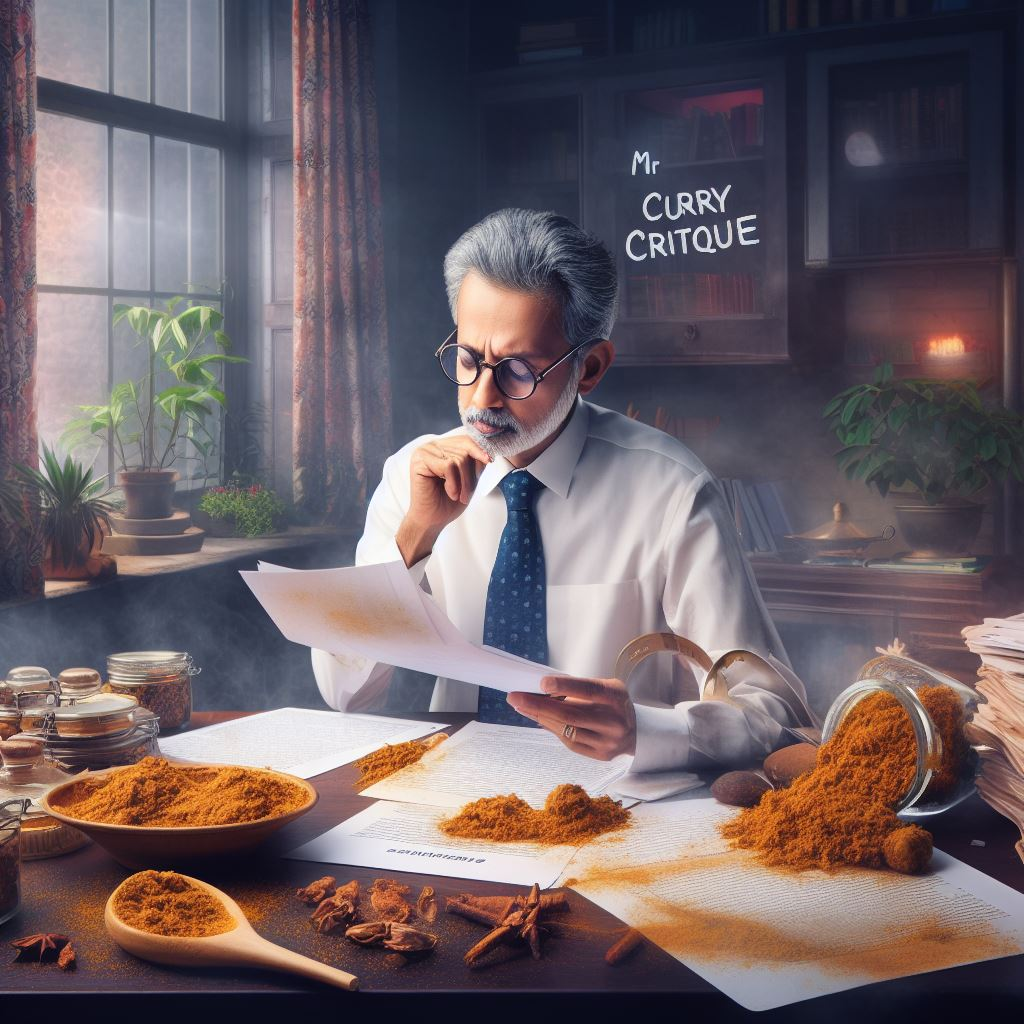
\includegraphics[width=\linewidth]{images/br_role_4}
            };
        \end{column}
        \begin{column}{0.5\textwidth}
            \begin{tcolorbox}[colback=white,colframe=codered,fonttitle=\bfseries, title=Dr. Curry Critique]
                The intriguing blend of Hamburg's historical trading routes and academia birthed Mr. Curry Critique. Analogizing spices to academic nuances, he finds himself immersed in the quest for that perfect scholarly recipe. A paper missing the academic 'spice' is often met with his critique, 'It lacks the zing!'.
            \end{tcolorbox}
        \end{column}
    \end{columns}
\end{frame}

\begin{frame}[plain]{Rejecting Reviewer}
    \begin{columns}
        \begin{column}{0.5\textwidth}
            \centering
            \tikz\node[inner sep=0pt, draw=none, drop shadow={shadow xshift=1mm,shadow yshift=-1mm,fill=black, opacity=0.3}]{
                
\includegraphics[width=\linewidth]{images/br_role_5}
            };
        \end{column}
        \begin{column}{0.5\textwidth}
            \begin{tcolorbox}[colback=white,colframe=codered,fonttitle=\bfseries, title=Ms. Bollywood Drama]
                A product of an exchange program between German universities and Bollywood's scriptwriting schools, Ms. Bollywood Drama seeks theatricality even in academia. To her, a paper isn't merely a collection of facts; it's an epic awaiting a dramatic twist. Lackluster submissions often earn her critique, `Needs more drama!'.
            \end{tcolorbox}
        \end{column}
    \end{columns}
\end{frame}

\begin{frame}[plain]{Rejecting Reviewer}
    \begin{columns}
        \begin{column}{0.5\textwidth}
            \centering
            \tikz\node[inner sep=0pt, draw=none, drop shadow={shadow xshift=1mm,shadow yshift=-1mm,fill=black, opacity=0.3}]{
                
\includegraphics[width=\linewidth]{images/br_role_6}
            };
        \end{column}
        \begin{column}{0.5\textwidth}
            \begin{tcolorbox}[colback=white,colframe=codered,fonttitle=\bfseries, title=Doktor Zu Kompliziert]
                In the hallowed corridors of Berlin's academies, Doktor Zu Kompliziert stands as a beacon of simplicity. Amidst the mire of overcomplexity, he's often the voice advocating for straightforwardness. Confronted with overwrought theories, his voice resounds, `Zu Kompliziert!' (Too Complicated).
            \end{tcolorbox}
        \end{column}
    \end{columns}
\end{frame}

\begin{frame}[plain]{Rejecting Reviewer}
    \begin{columns}
        \begin{column}{0.5\textwidth}
            \centering
            \tikz\node[inner sep=0pt, draw=none, drop shadow={shadow xshift=1mm,shadow yshift=-1mm,fill=black, opacity=0.3}]{
                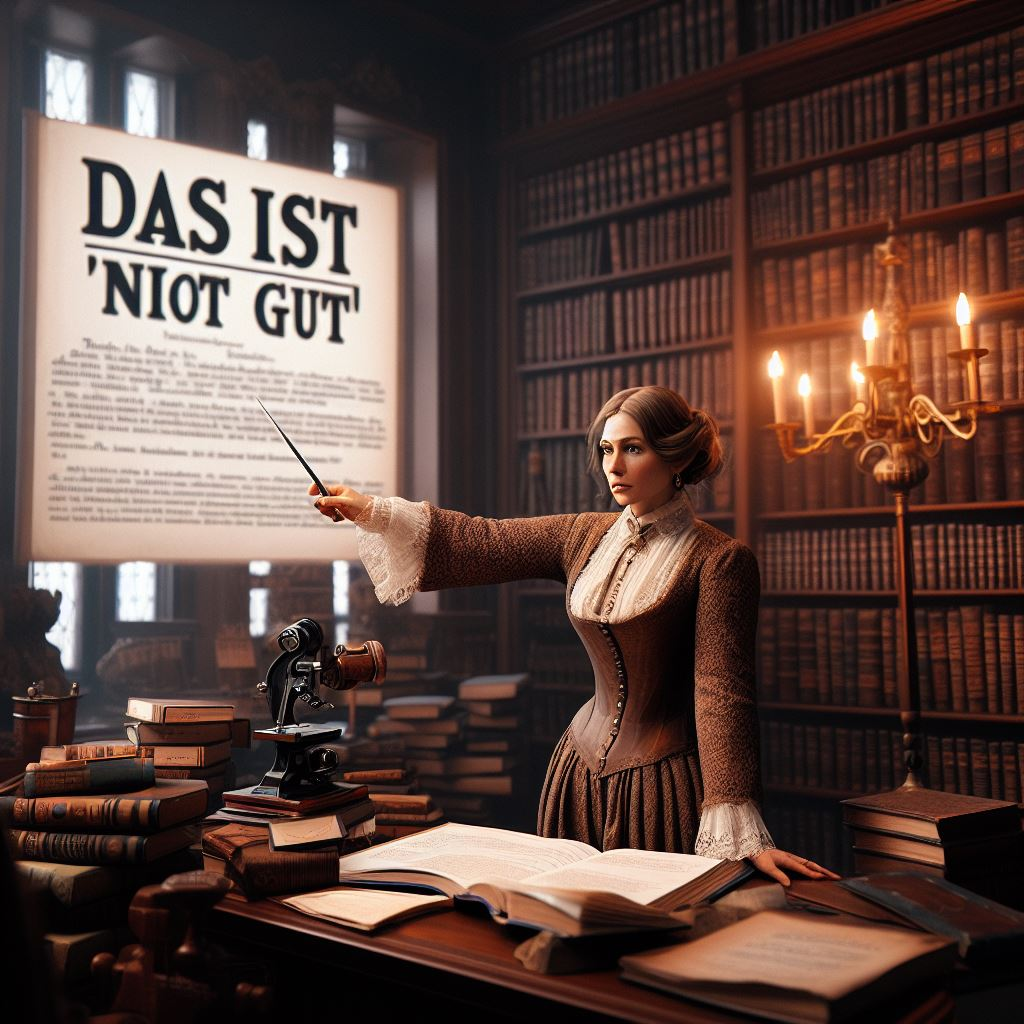
\includegraphics[width=\linewidth]{images/br_role_7}
            };
        \end{column}
        \begin{column}{0.5\textwidth}
            \begin{tcolorbox}[colback=white,colframe=codered,fonttitle=\bfseries, title=Madam Das Ist Nicht Gut]
                Hailing from an esteemed philosophy department in Düsseldorf, Madam Das Ist Nicht Gut is the epitome of rigorous academic critique. With every paper she reviews, she looks for that impeccable harmony of thought, akin to the perfect aesthetic. When the coherence wavers, she succinctly remarks, `Das ist nicht gut!' (That's not good).
            \end{tcolorbox}
        \end{column}
    \end{columns}
\end{frame}

\begin{frame}[plain]{Rejecting Reviewer}
    \begin{columns}
        \begin{column}{0.5\textwidth}
            \centering
            \tikz\node[inner sep=0pt, draw=none, drop shadow={shadow xshift=1mm,shadow yshift=-1mm,fill=black, opacity=0.3}]{
                
\includegraphics[width=\linewidth]{images/br_role_8}
            };
        \end{column}
        \begin{column}{0.5\textwidth}
            \begin{tcolorbox}[colback=white,colframe=codered,fonttitle=\bfseries, title=Herr `Nicht Genug Daten']
                A staunch believer in empirical evidence, he often finds himself reminiscing about the vastness of German skies, correlating it with his thirst for data in research papers. No amount of data seems satisfactory to him. He wandered through the corridors of academia, voicing the familiar lament, `Nicht genug Daten!' (Not enough data).
            \end{tcolorbox}
        \end{column}
    \end{columns}
\end{frame}

\begin{greenframe}[plain]{Accepting Reviewer}
    \begin{columns}
        \begin{column}{0.5\textwidth}
            \centering
            \tikz\node[inner sep=0pt, draw=none, drop shadow={shadow xshift=1mm,shadow yshift=-1mm,fill=black, opacity=0.3}]{
                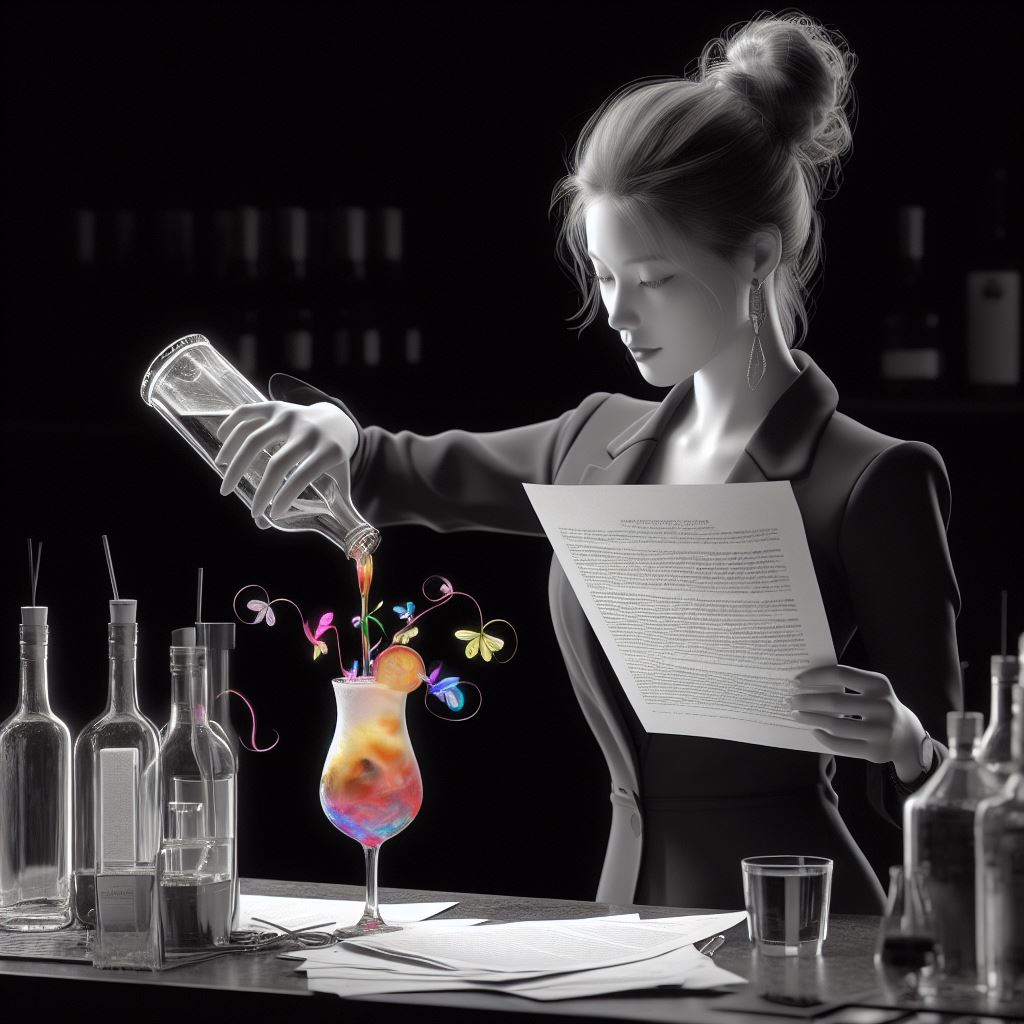
\includegraphics[width=\linewidth]{images/gr_role_1}
            };
        \end{column}
        \begin{column}{0.5\textwidth}
            \begin{tcolorbox}[colback=white,colframe=codegreen,fonttitle=\bfseries, title=Mixmaster Maddy]
                Maddy, a bartender-researcher, considers every paper a cocktail of ideas. She believes in blending theories smoothly. `Stir in a strong conclusion like a punchy cocktail!' she advises while pouring a vibrant concoction. Her reviews are both sharp and intoxicating.
            \end{tcolorbox}
        \end{column}
    \end{columns}
\end{greenframe}

\begin{greenframe}[plain]{Accepting Reviewer}
    \begin{columns}
        \begin{column}{0.5\textwidth}
            \centering
            \tikz\node[inner sep=0pt, draw=none, drop shadow={shadow xshift=1mm,shadow yshift=-1mm,fill=black, opacity=0.3}]{
                
\includegraphics[width=\linewidth]{images/gr_role_2}
            };
        \end{column}
        \begin{column}{0.5\textwidth}
            \begin{tcolorbox}[colback=white,colframe=codegreen,fonttitle=\bfseries, title=Checkout Charlie]
                Berlin's market kingpin, Charlie, is always on the lookout for hidden treasures in papers. `Found some sparkling insights!' he often exclaims. But, just like special offers at checkout, he believes every abstract needs a perk. `How about a dash of humor in the abstract?' he chuckles, scanning items with zest.
            \end{tcolorbox}
        \end{column}
    \end{columns}
\end{greenframe}

\begin{greenframe}[plain]{Accepting Reviewer}
    \begin{columns}
        \begin{column}{0.5\textwidth}
            \centering
            \tikz\node[inner sep=0pt, draw=none, drop shadow={shadow xshift=1mm,shadow yshift=-1mm,fill=black, opacity=0.3}]{
                
\includegraphics[width=\linewidth]{images/gr_role_3}
            };
        \end{column}
        \begin{column}{0.5\textwidth}
            \begin{tcolorbox}[colback=white,colframe=codegreen,fonttitle=\bfseries, title=Kebab King]
                The döner maestro, this man doesn't just wrap kebabs, he wraps praise and critiques together seamlessly. `Such fiery research needs--salate alles und alles drei soße!' he often suggests. Serving sizzling reviews is his forte, often sandwiched with hearty encouragement.
            \end{tcolorbox}
        \end{column}
    \end{columns}
\end{greenframe}

\begin{greenframe}[plain]{Accepting Reviewer}
    \begin{columns}
        \begin{column}{0.5\textwidth}
            \centering
            \tikz\node[inner sep=0pt, draw=none, drop shadow={shadow xshift=1mm,shadow yshift=-1mm,fill=black, opacity=0.3}]{
                
\includegraphics[width=\linewidth]{images/gr_role_4}
            };
        \end{column}
        \begin{column}{0.5\textwidth}
            \begin{tcolorbox}[colback=white,colframe=codegreen,fonttitle=\bfseries, title=Bavarian Brigitte]
                Brigitte, with her classic Bavarian spirit, resonates with Oktoberfest vibes all year round. For her, every commendable paper deserves a hearty `Prost!' With braided hair, traditional dirndl, and infectious enthusiasm, she often says, `Such brilliance! More of this, and the academic world will dance in joy!'
            \end{tcolorbox}
        \end{column}
    \end{columns}
\end{greenframe}

\begin{greenframe}[plain]{Accepting Reviewer}
    \begin{columns}
        \begin{column}{0.5\textwidth}
            \centering
            \tikz\node[inner sep=0pt, draw=none, drop shadow={shadow xshift=1mm,shadow yshift=-1mm,fill=black, opacity=0.3}]{
                
\includegraphics[width=\linewidth]{images/gr_role_5}
            };
        \end{column}
        \begin{column}{0.5\textwidth}
            \begin{tcolorbox}[colback=white,colframe=codegreen,fonttitle=\bfseries, title=Positive Pete]
                Paderborn's pride, Pete's reviews always carry a hint of the historic charm of his hometown. Overflowing with optimism, Pete looks for the silver lining in every research cloud. `Almost there! Just a touch of old-world wisdom will elevate this,' he often remarks, with Paderborn's majestic skyline in his heart.
            \end{tcolorbox}
        \end{column}
    \end{columns}
\end{greenframe}

\begin{greenframe}[plain]{Accepting Reviewer}
    \begin{columns}
        \begin{column}{0.5\textwidth}
            \centering
            \tikz\node[inner sep=0pt, draw=none, drop shadow={shadow xshift=1mm,shadow yshift=-1mm,fill=black, opacity=0.3}]{
                
\includegraphics[width=\linewidth]{images/gr_role_6}
            };
        \end{column}
        \begin{column}{0.5\textwidth}
            \begin{tcolorbox}[colback=white,colframe=codegreen,fonttitle=\bfseries, title=Techie Ramesh]
                Ramesh, once Bangalore's IT jewel, now dives deep into academia. He's a bridge between traditional wisdom and modern insights. `Your tech approach is impeccable, but can we weave in some age-old Indian ethos?' he suggests, ever so often. Merging modernity with tradition is his reviewing mantra.
            \end{tcolorbox}
        \end{column}
    \end{columns}
\end{greenframe}

\begin{greenframe}[plain]{Accepting Reviewer}
    \begin{columns}
        \begin{column}{0.5\textwidth}
            \centering
            \tikz\node[inner sep=0pt, draw=none, drop shadow={shadow xshift=1mm,shadow yshift=-1mm,fill=black, opacity=0.3}]{
                
\includegraphics[width=\linewidth]{images/gr_role_7}
            };
        \end{column}
        \begin{column}{0.5\textwidth}
            \begin{tcolorbox}[colback=white,colframe=codegreen,fonttitle=\bfseries, title=Guidance Guru]
                Dwelling under the banyan's shade, this Indian spiritualist reads beyond mere words. `The cosmic energy of your paper resonates with ancient vibrations,' he'd muse. He feels every paper should be rooted in age-old wisdom. `Perhaps blend in some tangible facts to ground this ethereal energy?' is his sage advice.
            \end{tcolorbox}
        \end{column}
    \end{columns}
\end{greenframe}

\begin{greenframe}[plain]{Accepting Reviewer}
    \begin{columns}
        \begin{column}{0.5\textwidth}
            \centering
            \tikz\node[inner sep=0pt, draw=none, drop shadow={shadow xshift=1mm,shadow yshift=-1mm,fill=black, opacity=0.3}]{
                
\includegraphics[width=\linewidth]{images/gr_role_8}
            };
        \end{column}
        \begin{column}{0.5\textwidth}
            \begin{tcolorbox}[colback=white,colframe=codegreen,fonttitle=\bfseries, title=Priestly Perspectives]
                Stationed in an Italian cathedral, our father finds divinity in every draft. `Your ideas seem touched by the divine. How about a revelation in the results?' he often suggests. Holding a rosary, he believes every paper, just like souls, deserves redemption and a chance to shine in academic heavens.
            \end{tcolorbox}
        \end{column}
    \end{columns}
\end{greenframe}

\end{document}
